%%%%%%%%%%%%%%%%%%%%%%%%%%%%%%%%%%%%%%%%%%%%%%%%%%%%%%%%%%%%%%%%%%%%%%%%%%%%%%%%%%%%%%%%%%%%%%

%%%%%%%%%%%%%%%%%%%%%%%%%%%%%%%%%%%%%%%%%%%%%%%%%%%%%%%%%%%%%%%%%%%%%%%%%%%%%%%%%%%%%%%%%%%%%% 

%\documentclass{beamer} %voce pode usar este modelo tambem
\documentclass[handout,t]{beamer}
\usepackage{graphicx,url}
\usepackage[brazil]{babel}   
\usepackage[utf8]{inputenc}
\batchmode
% \usepackage{pgfpages}
% \pgfpagesuselayout{4 on 1}[letterpaper,landscape,border shrink=5mm]
\usepackage{amsmath,amssymb,enumerate,epsfig,bbm,calc,color,ifthen,capt-of}
\usetheme{Berlin}
\usecolortheme{whale}

%-------------------------Title information------------------------------------------------
\title[Where and why are temperature forecasts faulty?]{Where and why are temperature forecasts faulty?}
\subtitle{Data Expo 2018}
\date{July 30, 2018}
\author[Matt Higham, Erin Howard]{Matt Higham \\ Erin Howard}

%-------------------------Logo na parte de baixo do slide------------------------------------------
\pgfdeclareimage[height=1.5cm]{senac-logo}{logo.pdf}
\logo{\pgfuseimage{senac-logo}\hspace*{0.5cm}\vspace*{-0.5cm}}

%-------------------------Este código faz o menuzinho bacana na parte superior do slide------------
%\AtBeginSection[]
%{
%  \begin{frame}<beamer>
%    \frametitle{Outline}
%    \tableofcontents[currentsection]
%  \end{frame}
%}
\beamerdefaultoverlayspecification{<+->}
% -----------------------------------------------------------------------------
\begin{document}
% -----------------------------------------------------------------------------

%------------------------------------------------------------
\frame{\titlepage}
\section{}
\begin{frame}{Do weather forecasts systematically bias temperature predictions?}

  \hspace*{-0.5cm}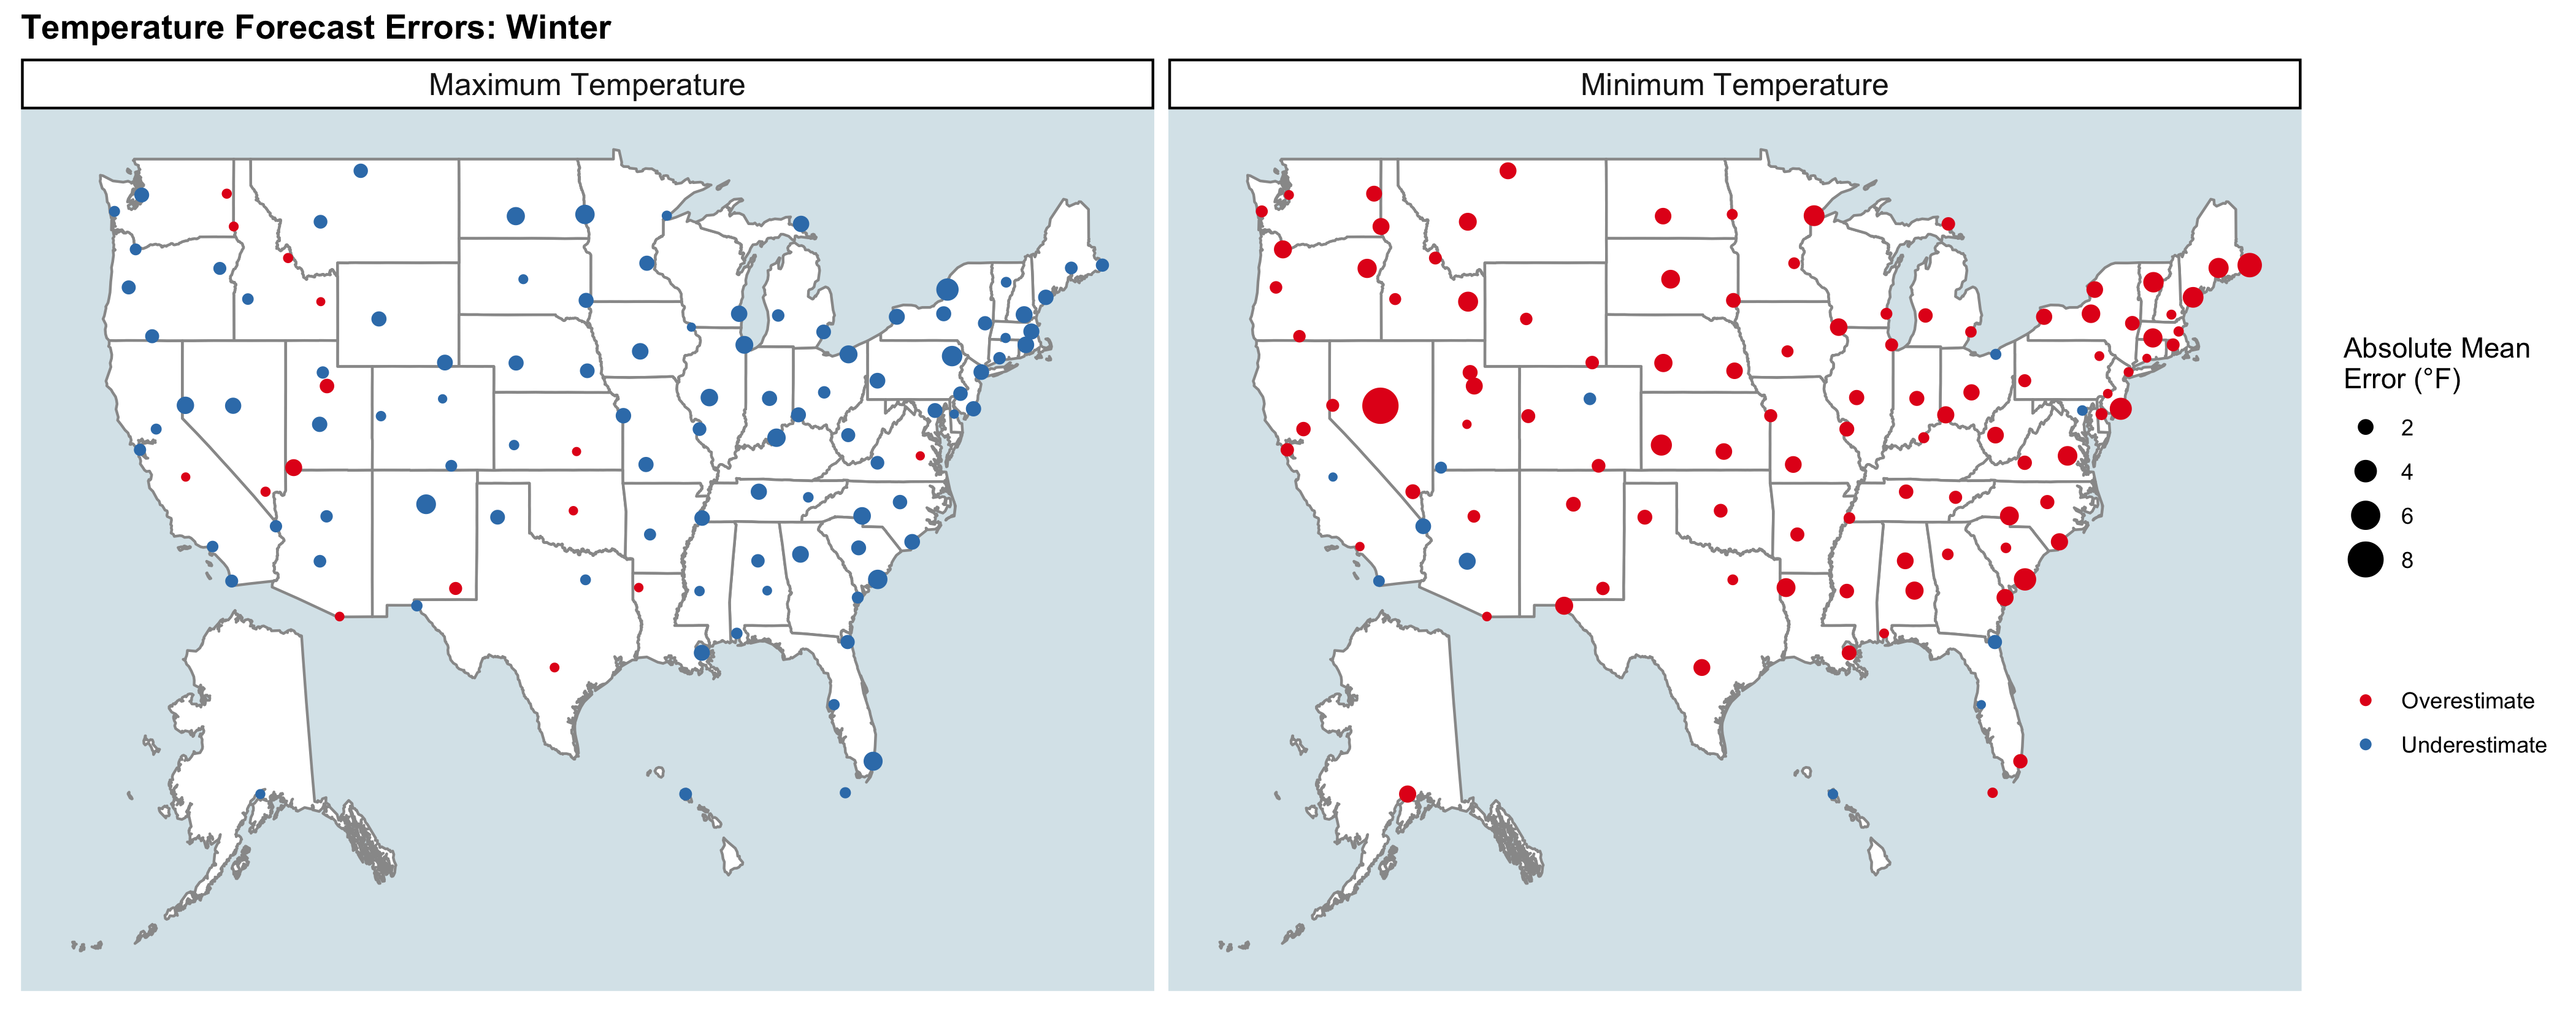
\includegraphics[width=1.1\textwidth,natwidth=200,natheight=87]{Both_winter_maps_new.png}
  %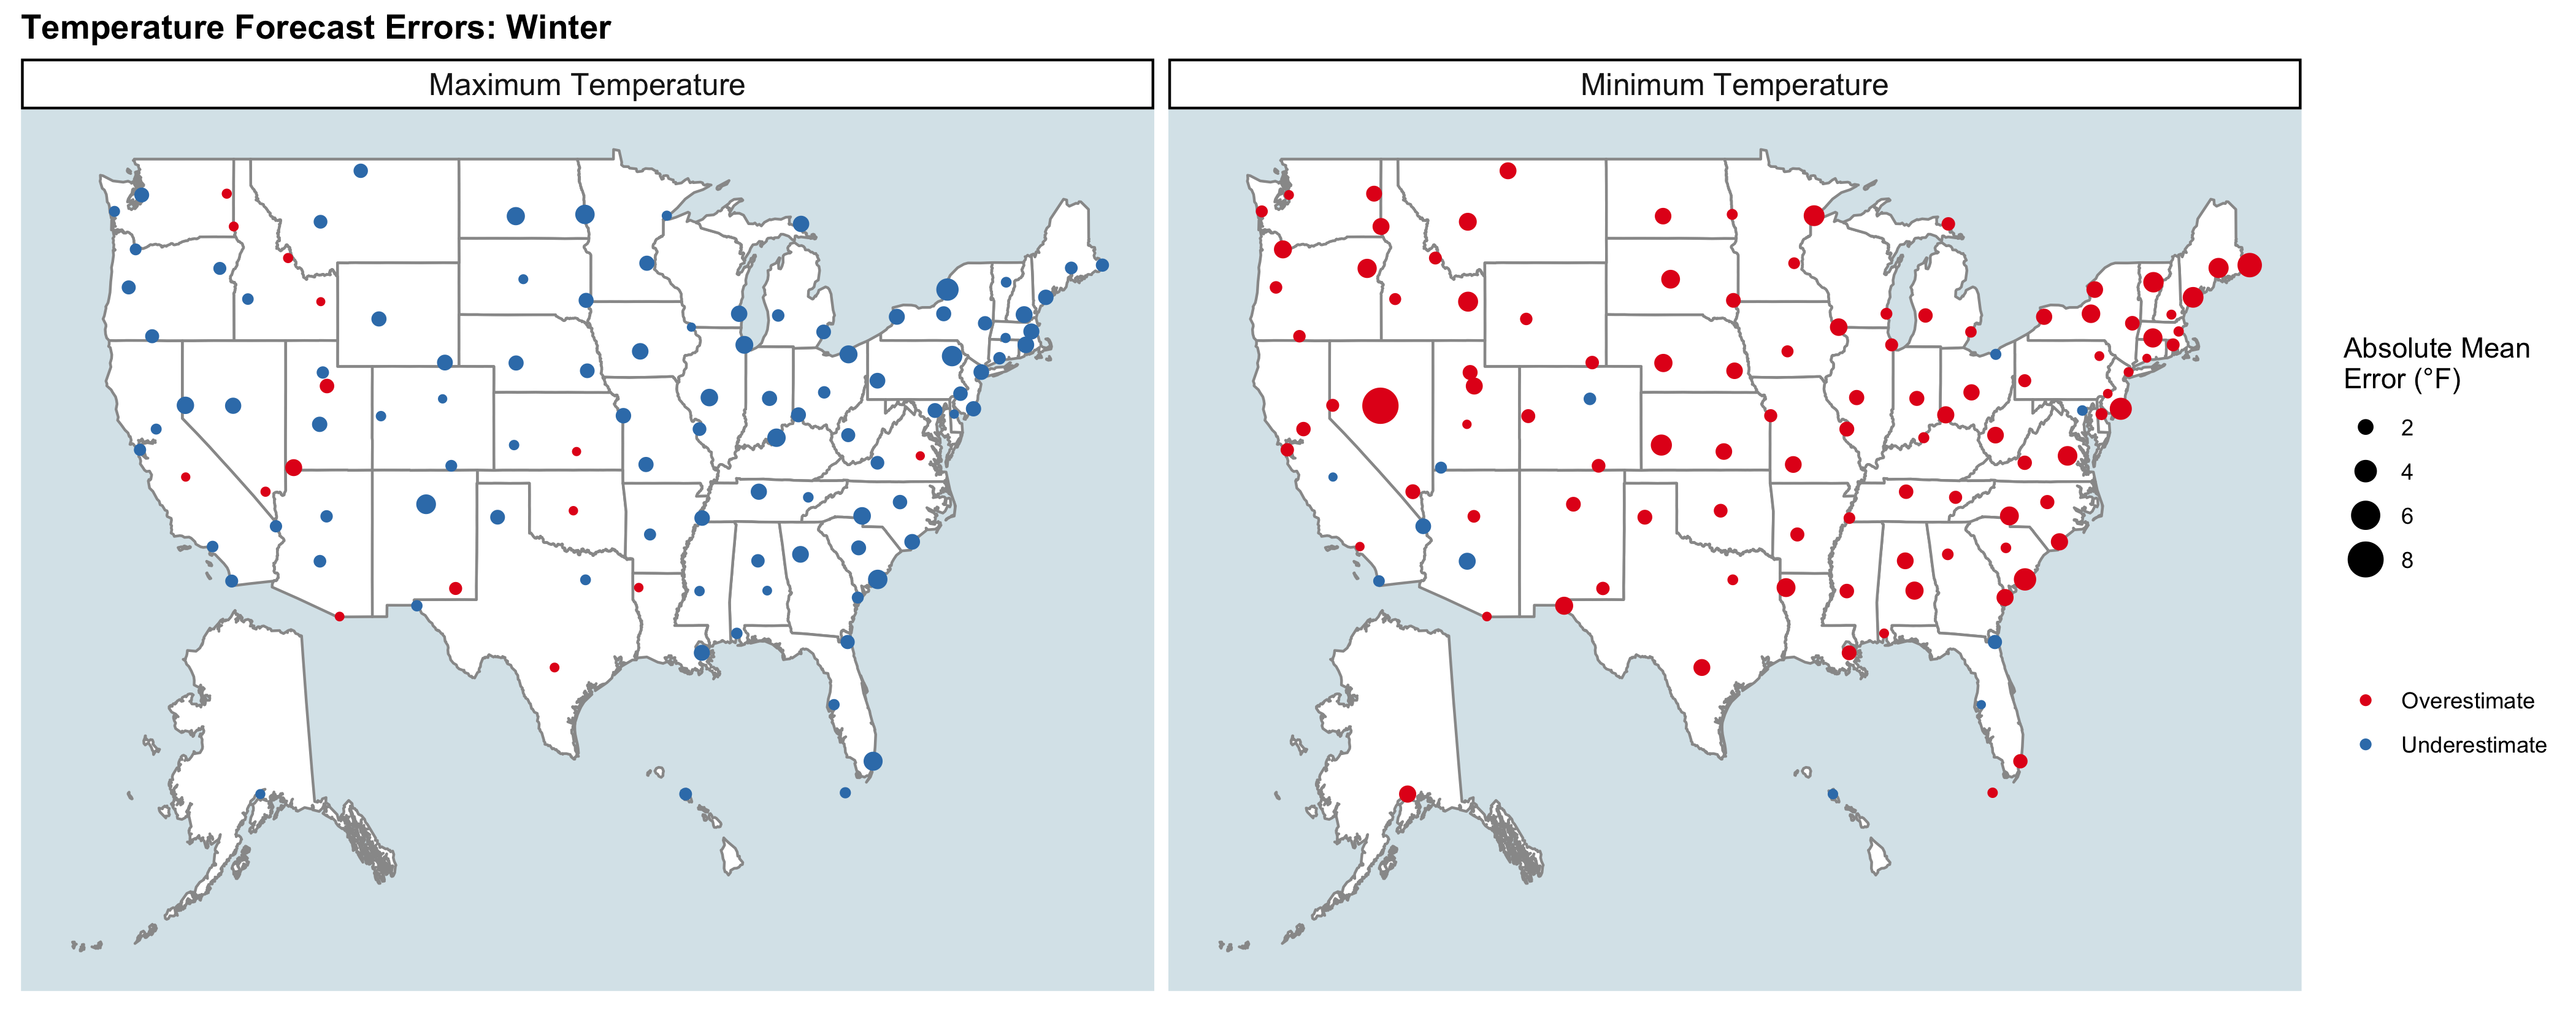
\includegraphics[scale=0.08]{Both_winter_maps_new.png}

\end{frame}



% -----------------------------------------------------------------------------
\section{}
\begin{frame}{Might the bias come from misalignment in the airport historical data and the city center forecasts?}
  \begin{center}
  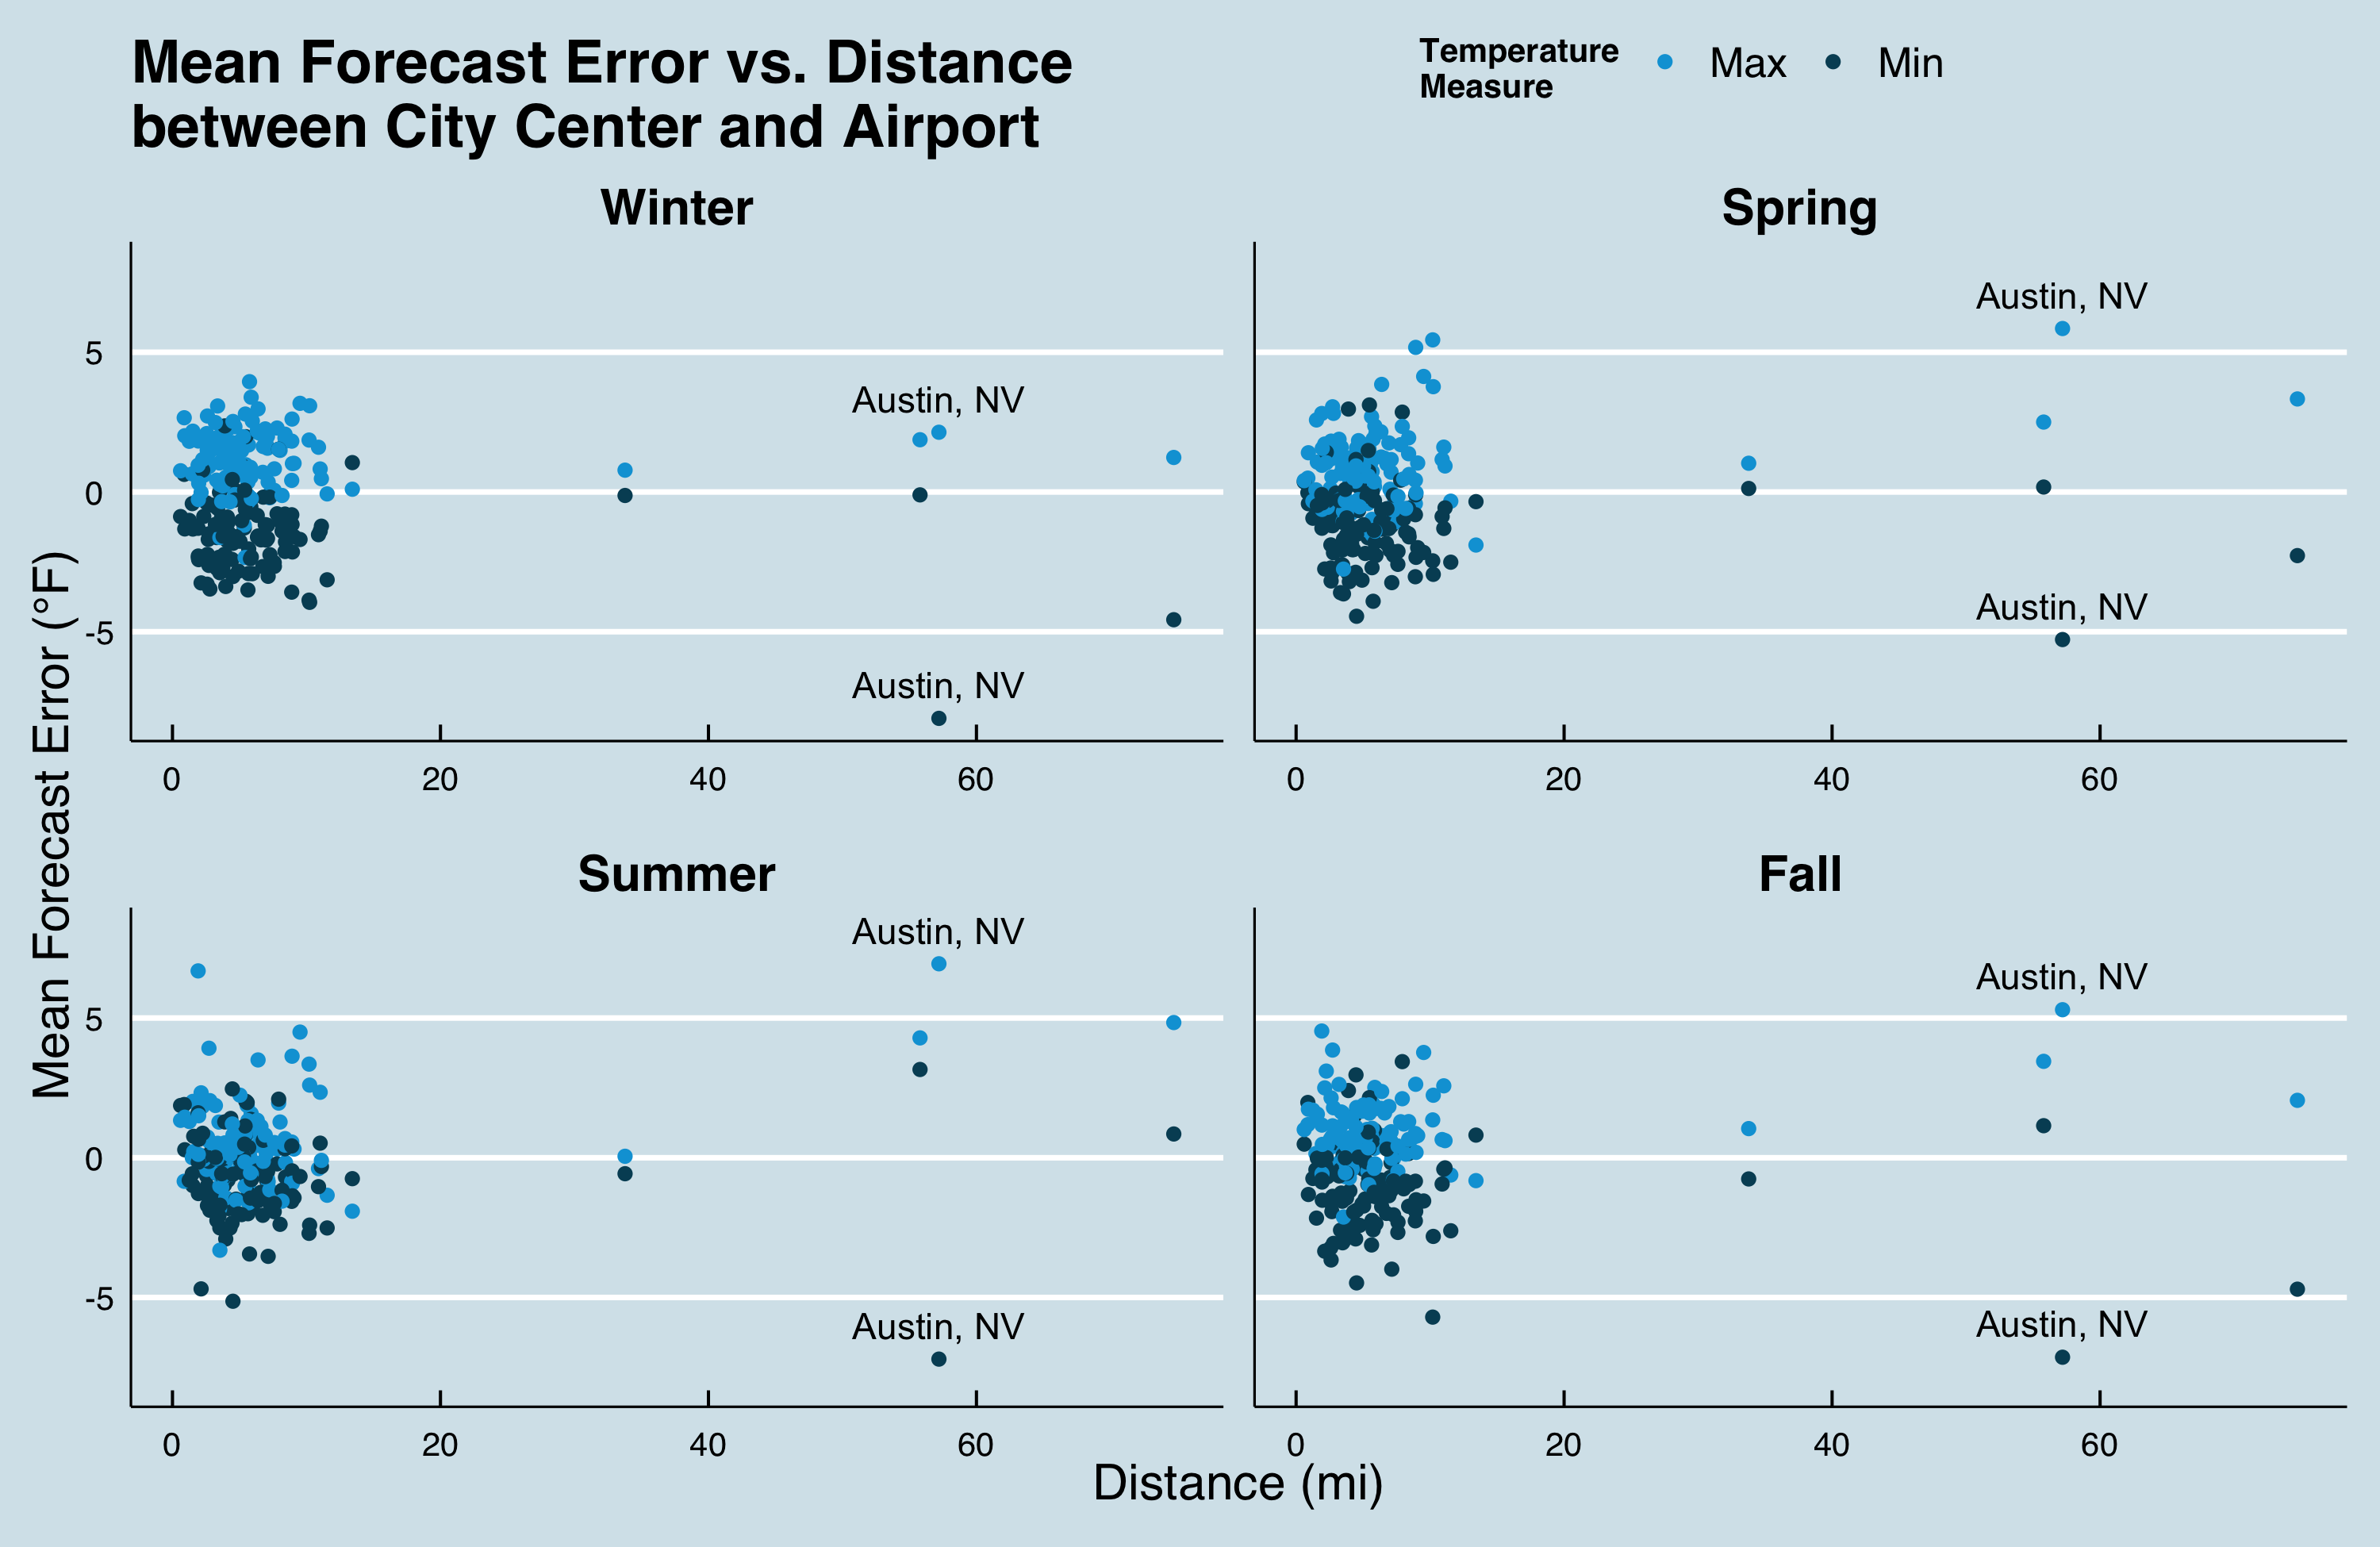
\includegraphics[scale=0.07]{Distance_Plot_Poster_new.png}
  \end{center}
\end{frame}
%------------------------------------------------------------------------------

%------------------------------------------------------------------------------
\section{}
\begin{frame}{Are cities' prediction errors large due to bias or variance? Does this depend on the city?
}
  \begin{center}
  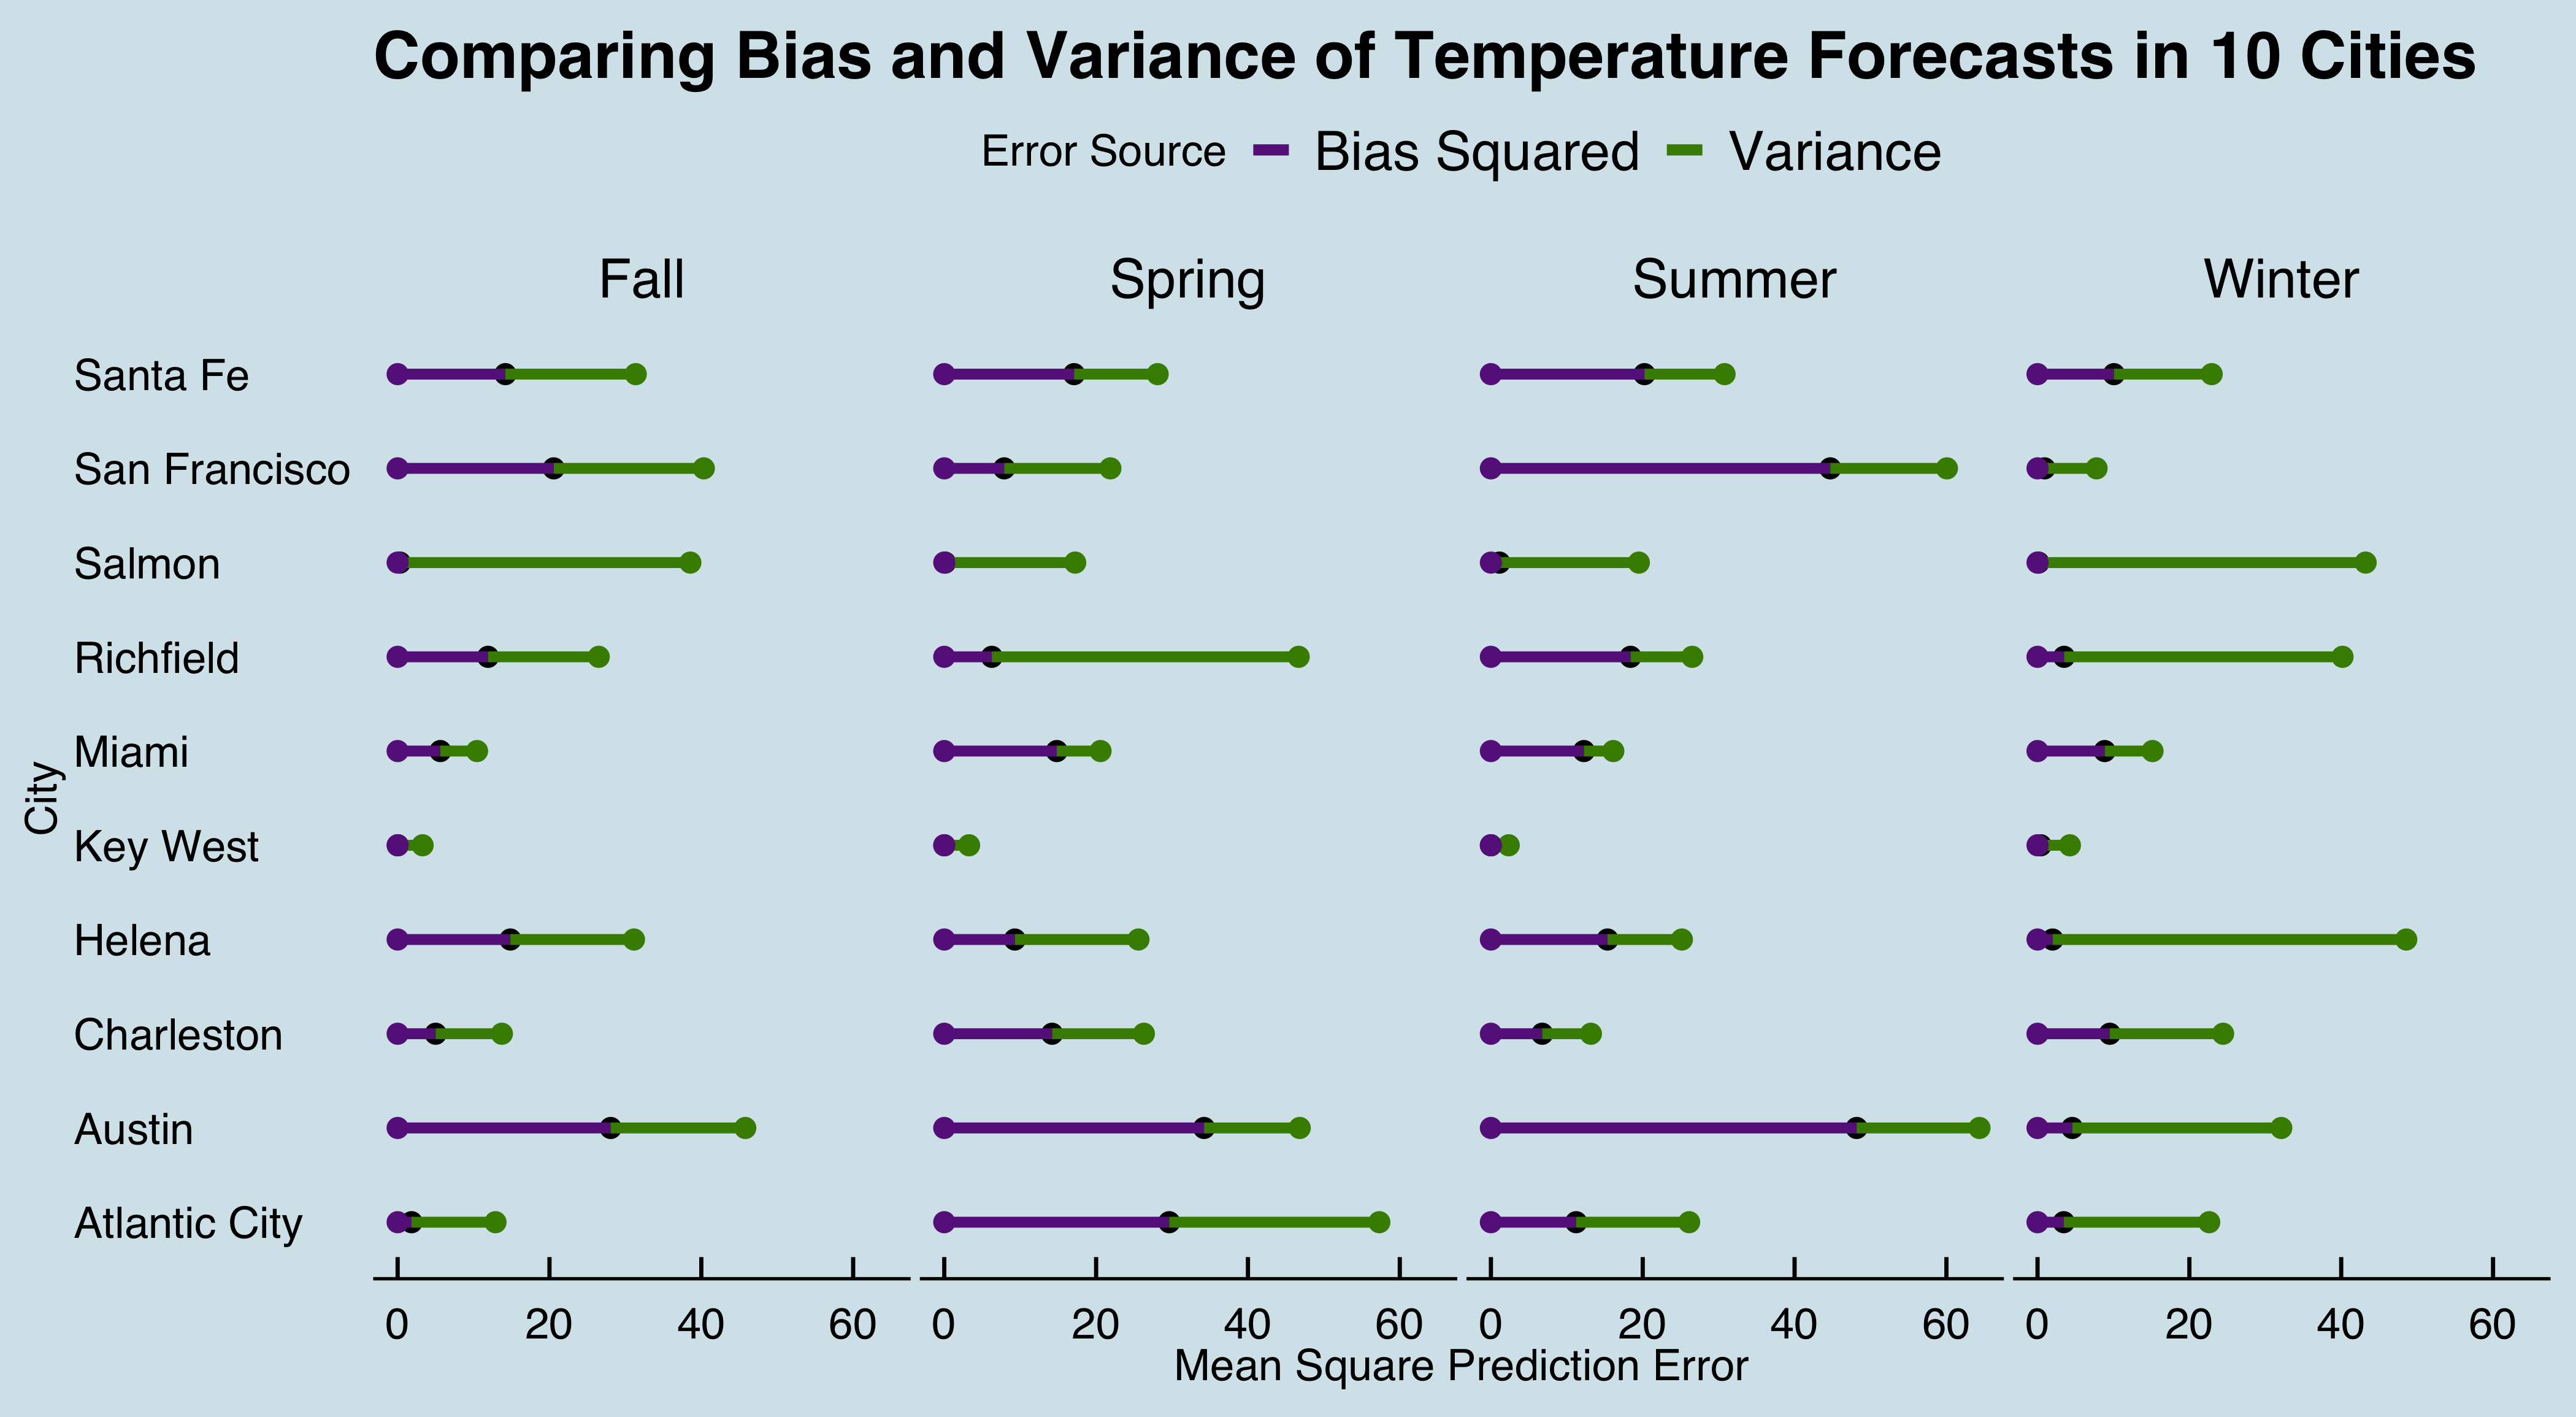
\includegraphics[scale=0.06]{BiasVarGraph.png}
  \end{center}
\end{frame}
%------------------------------------------------------------------------------




\end{document}
%------------------------------------------------------------------------------